\chapter{ベンチマーク}
\label{chap_Results}

\section{環境}

ベンチマークの実行環境を,
表\ref{table_env}に示す.

\begin{table}[hbtp]
  \label{table_env}
  \begin{center}
    \caption{実行環境}
    \begin{tabular}{cc} \hline
      Component & Type \rule[0pt]{0pt}{0pt} \\ \hline
      CPU & AMD Ryzen7 1700 (8Cores/16Threads) \rule[0pt]{0pt}{0pt} \\ 
      & Base Clock 3GHz / Max Boost Clock 3.7GHz \rule[0pt]{0pt}{0pt} \\
      & Total L1 Cache: 768KB / Total L2 Cache: 4MB / Total L3 Cache: 16MB \\
      Memory & DDR4-2666 32GB \rule[0pt]{0pt}{0pt} \\
      OS & Ubuntu 16.04 LTS \rule[0pt]{0pt}{0pt} \\
      Compiler & gcc version 5.4.0 20160609 (Ubuntu 5.4.0-6ubuntu1~16.04.11) \rule[0pt]{0pt}{0pt} \\ \hline
    \end{tabular}
  \end{center}
\end{table}


\section{結果}

{\bf Loadfactor}

{\bf メモリ使用量}

{\bf 挿入}

{\bf 探査}

{\bf 削除}

\begin{figure}[h]
  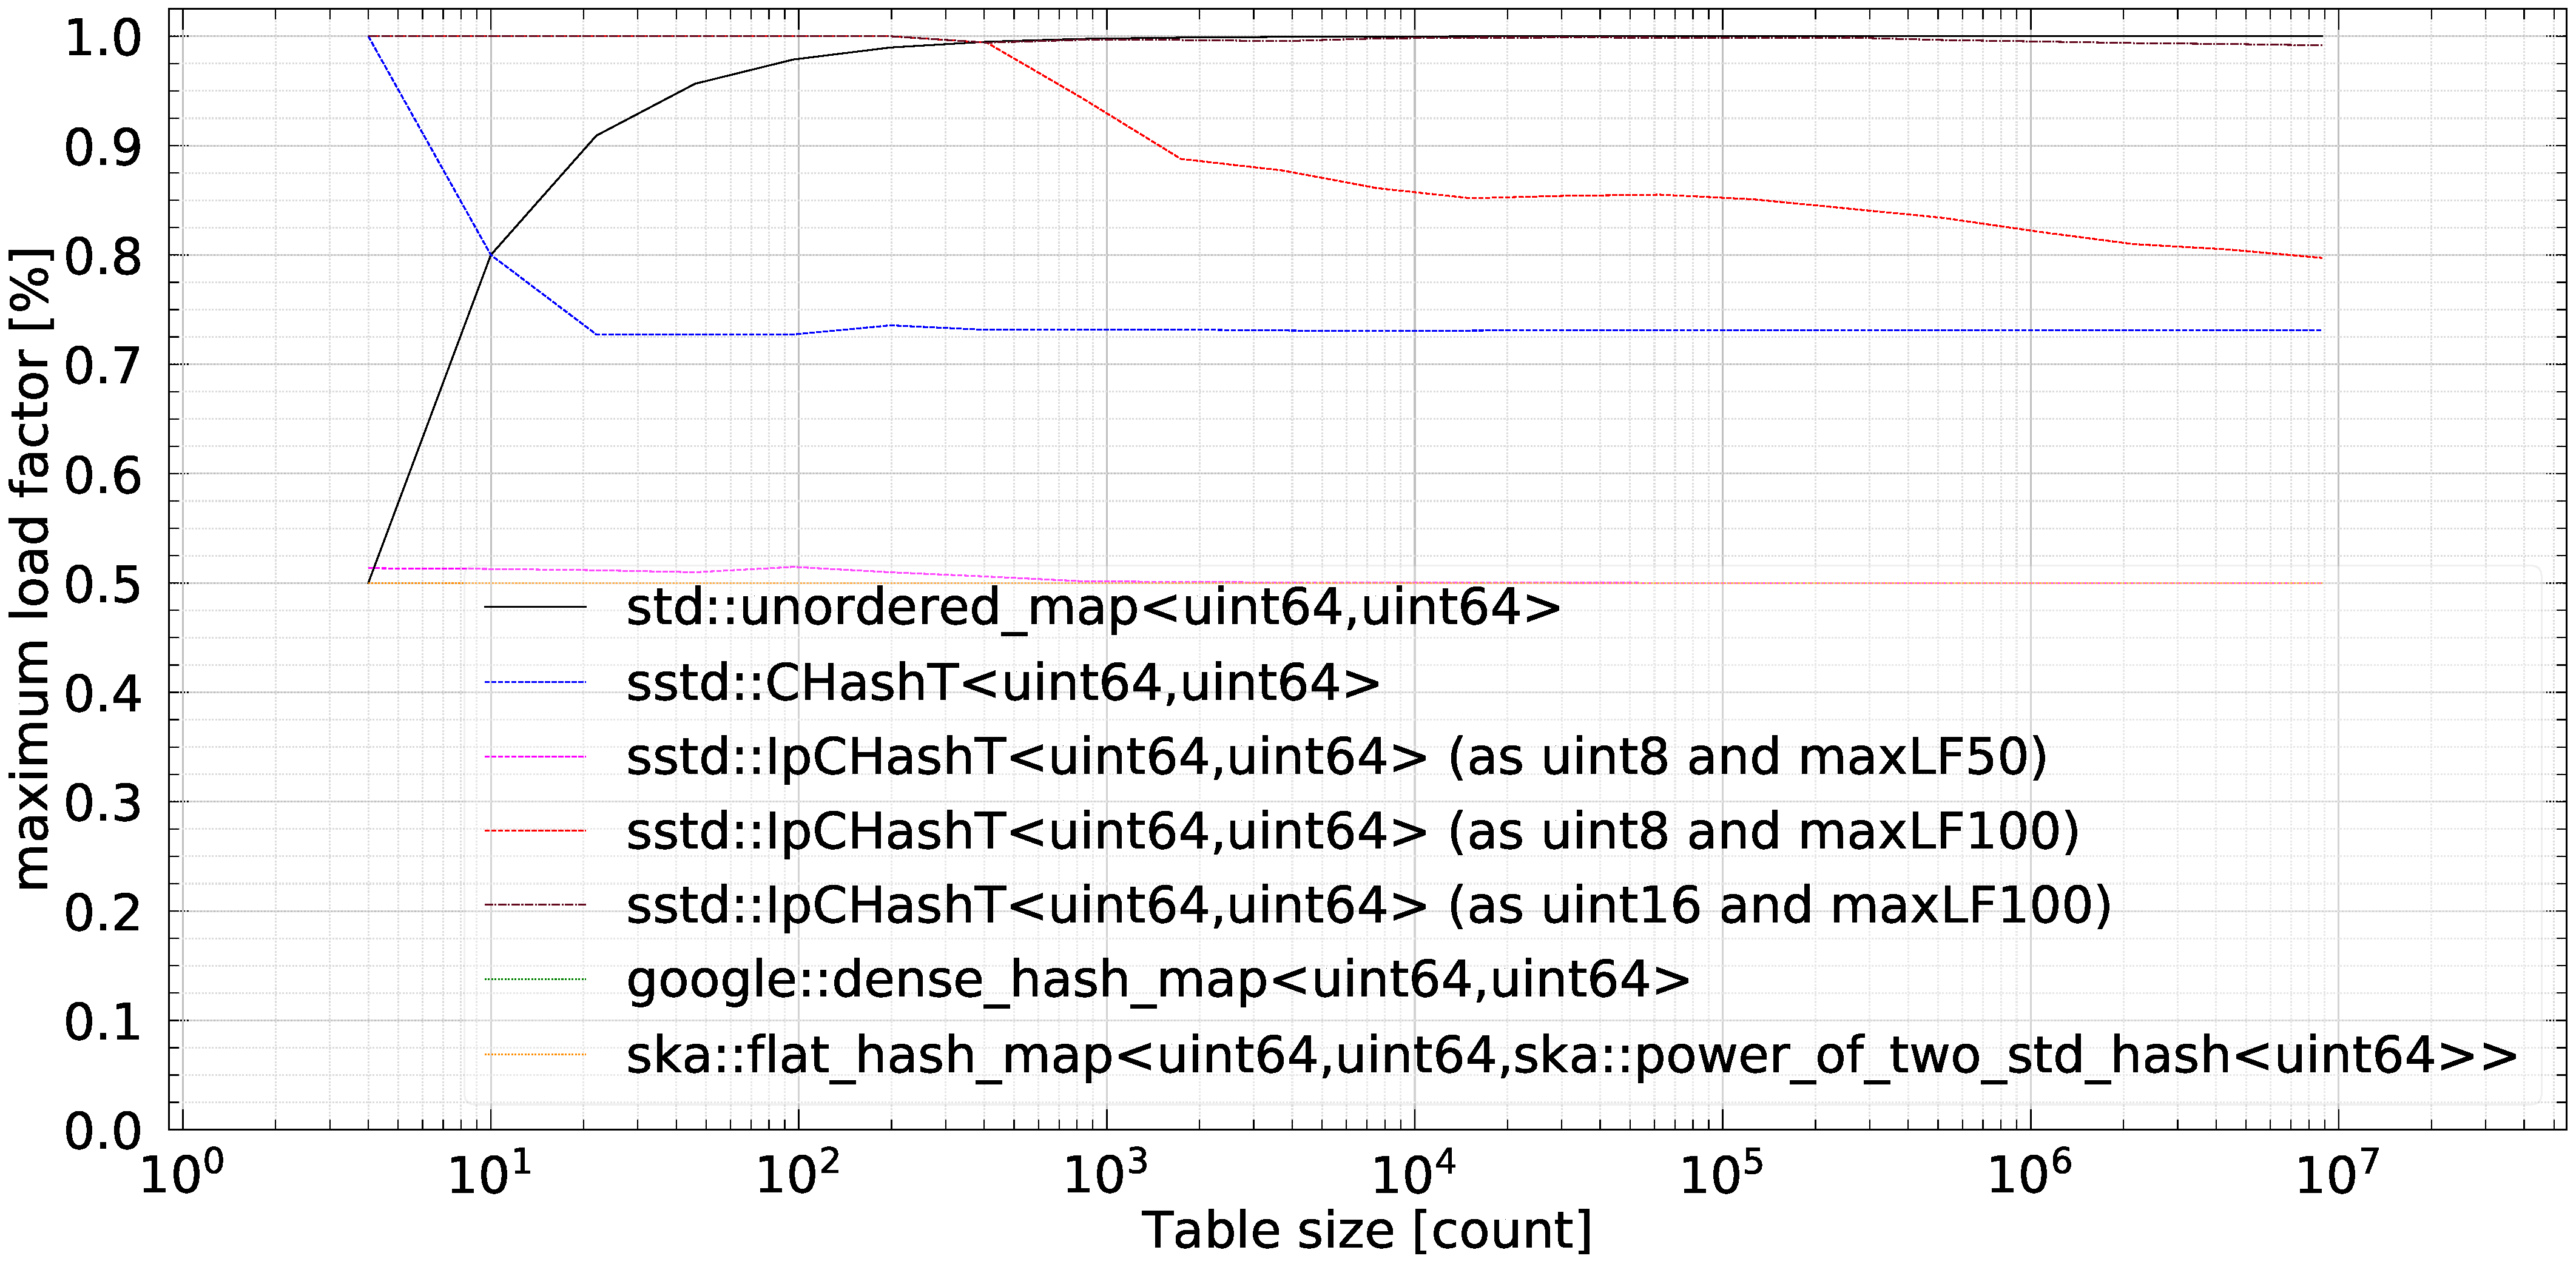
\includegraphics[scale=0.24]{./fig_bench/maxLoadFactor_med.pdf}
  \caption{
    Maximum load factor. Maximum load factor of std::IpHashT is limitted by its maximum length of shift\_T.
    Maximum load factor of google::dense\_hash\_map is artificially limited by 50 \%.
  }
  \label{fig_bench_LF}
\end{figure}

\begin{figure}[h]
  \hspace{-1mm}
  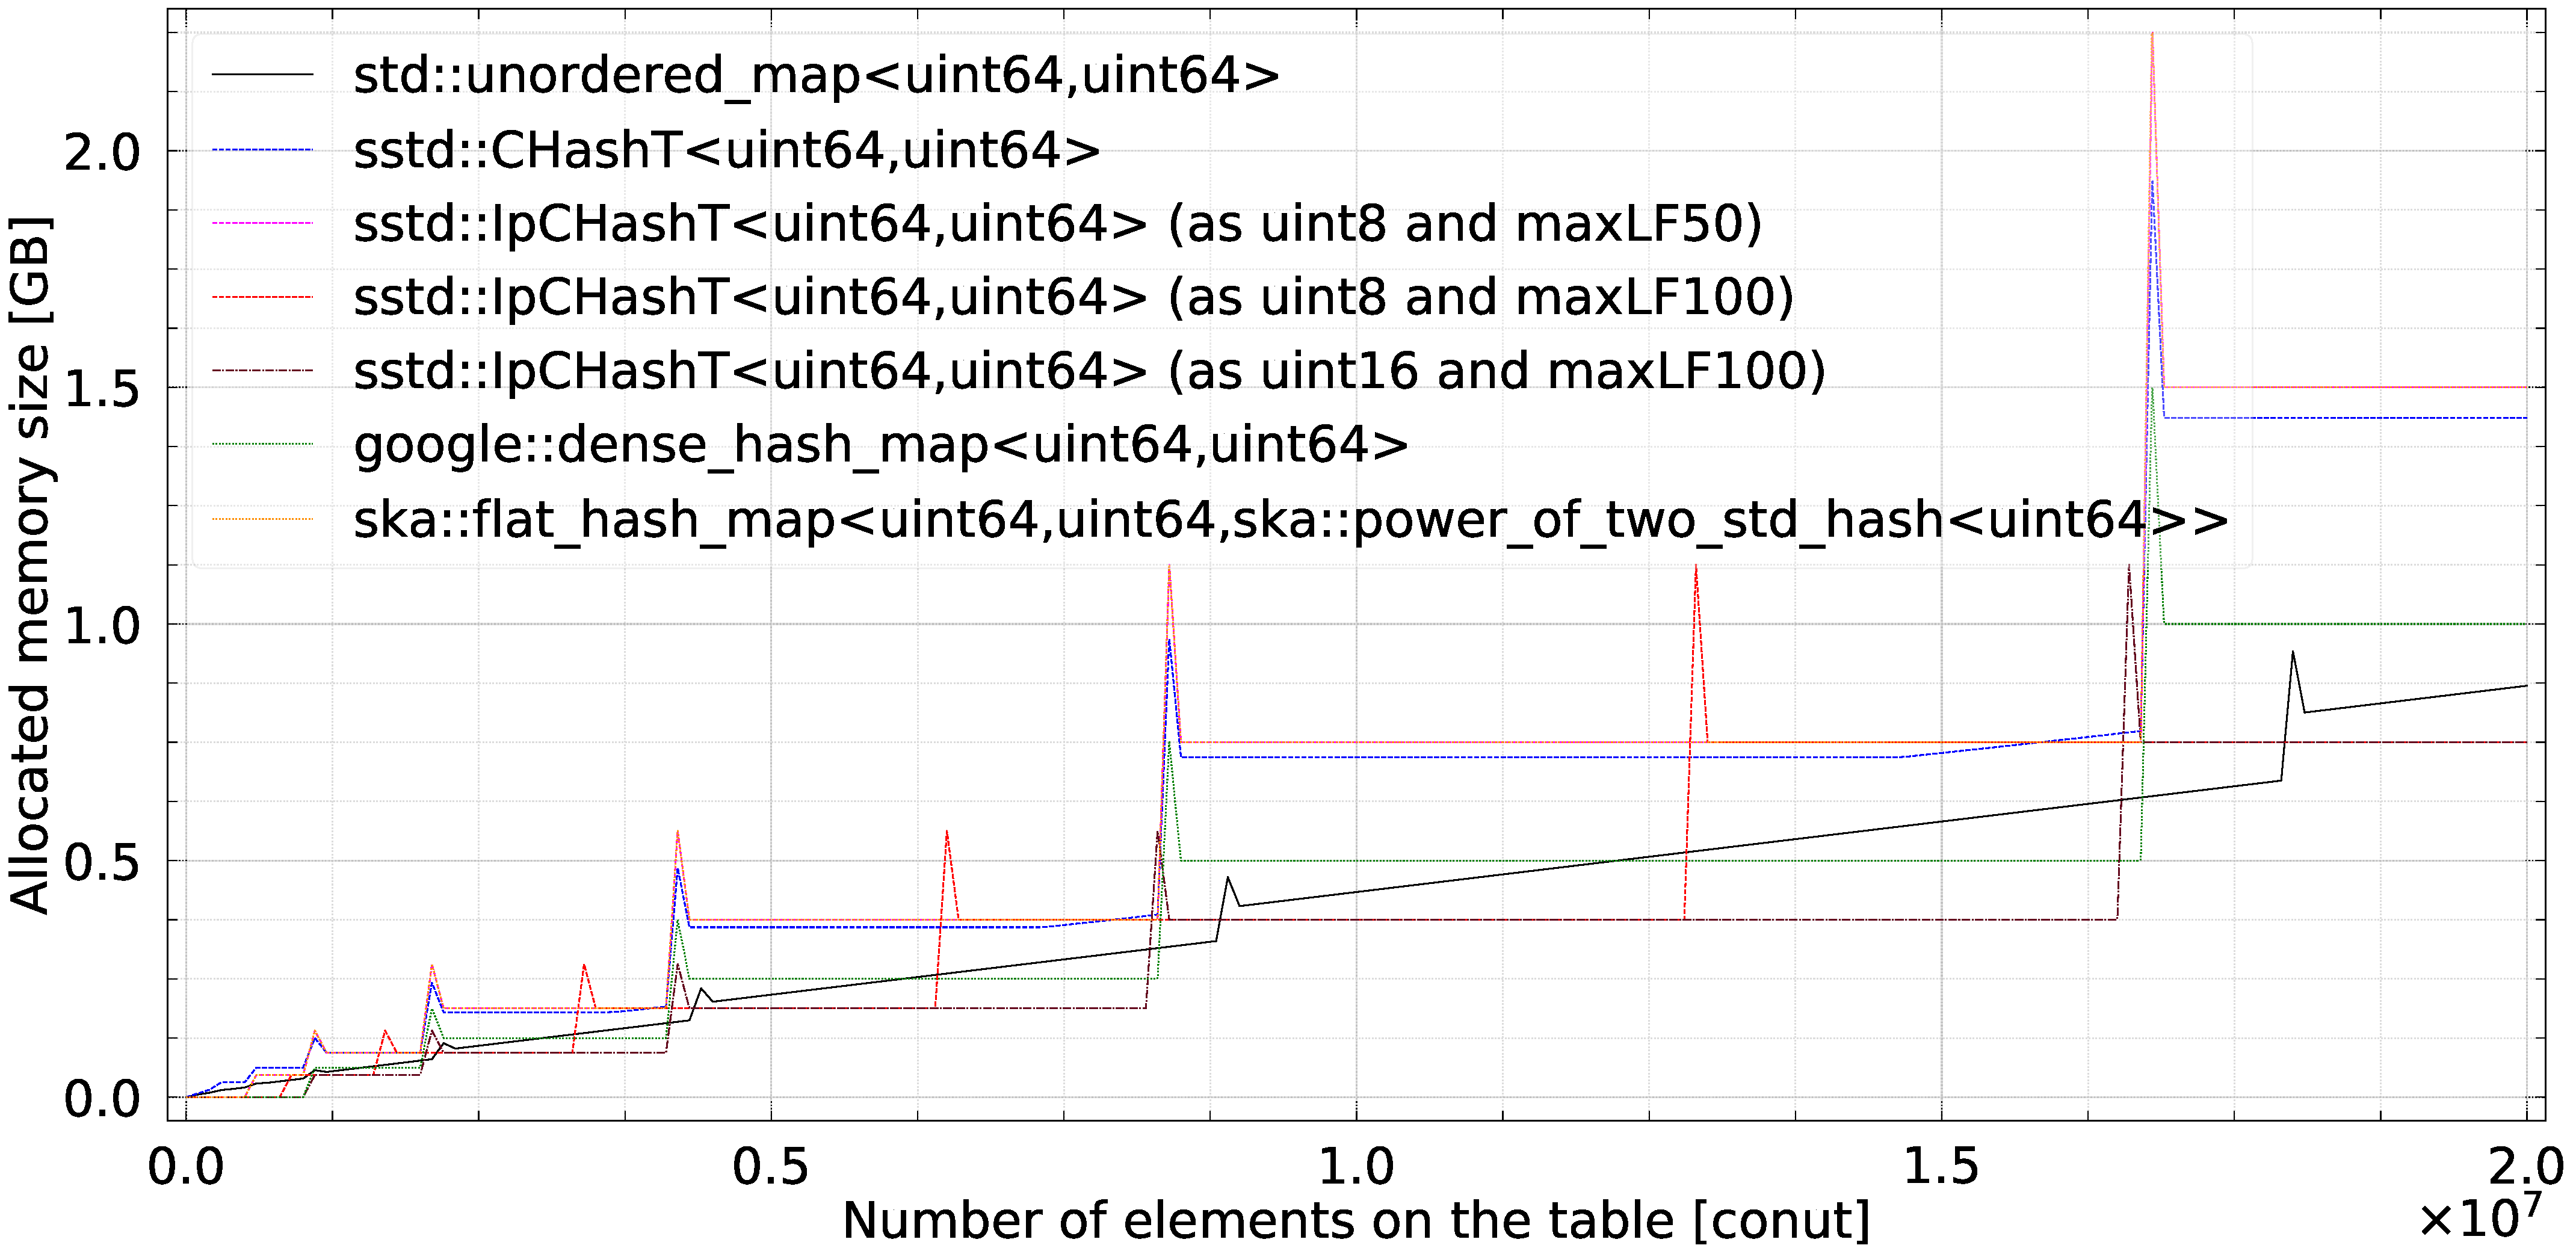
\includegraphics[scale=0.24]{./fig_bench/usedMemory.pdf}
  \caption{ Allocated memory size. }
  \label{fig_bench_memory}
\end{figure}

\begin{figure}[h]
  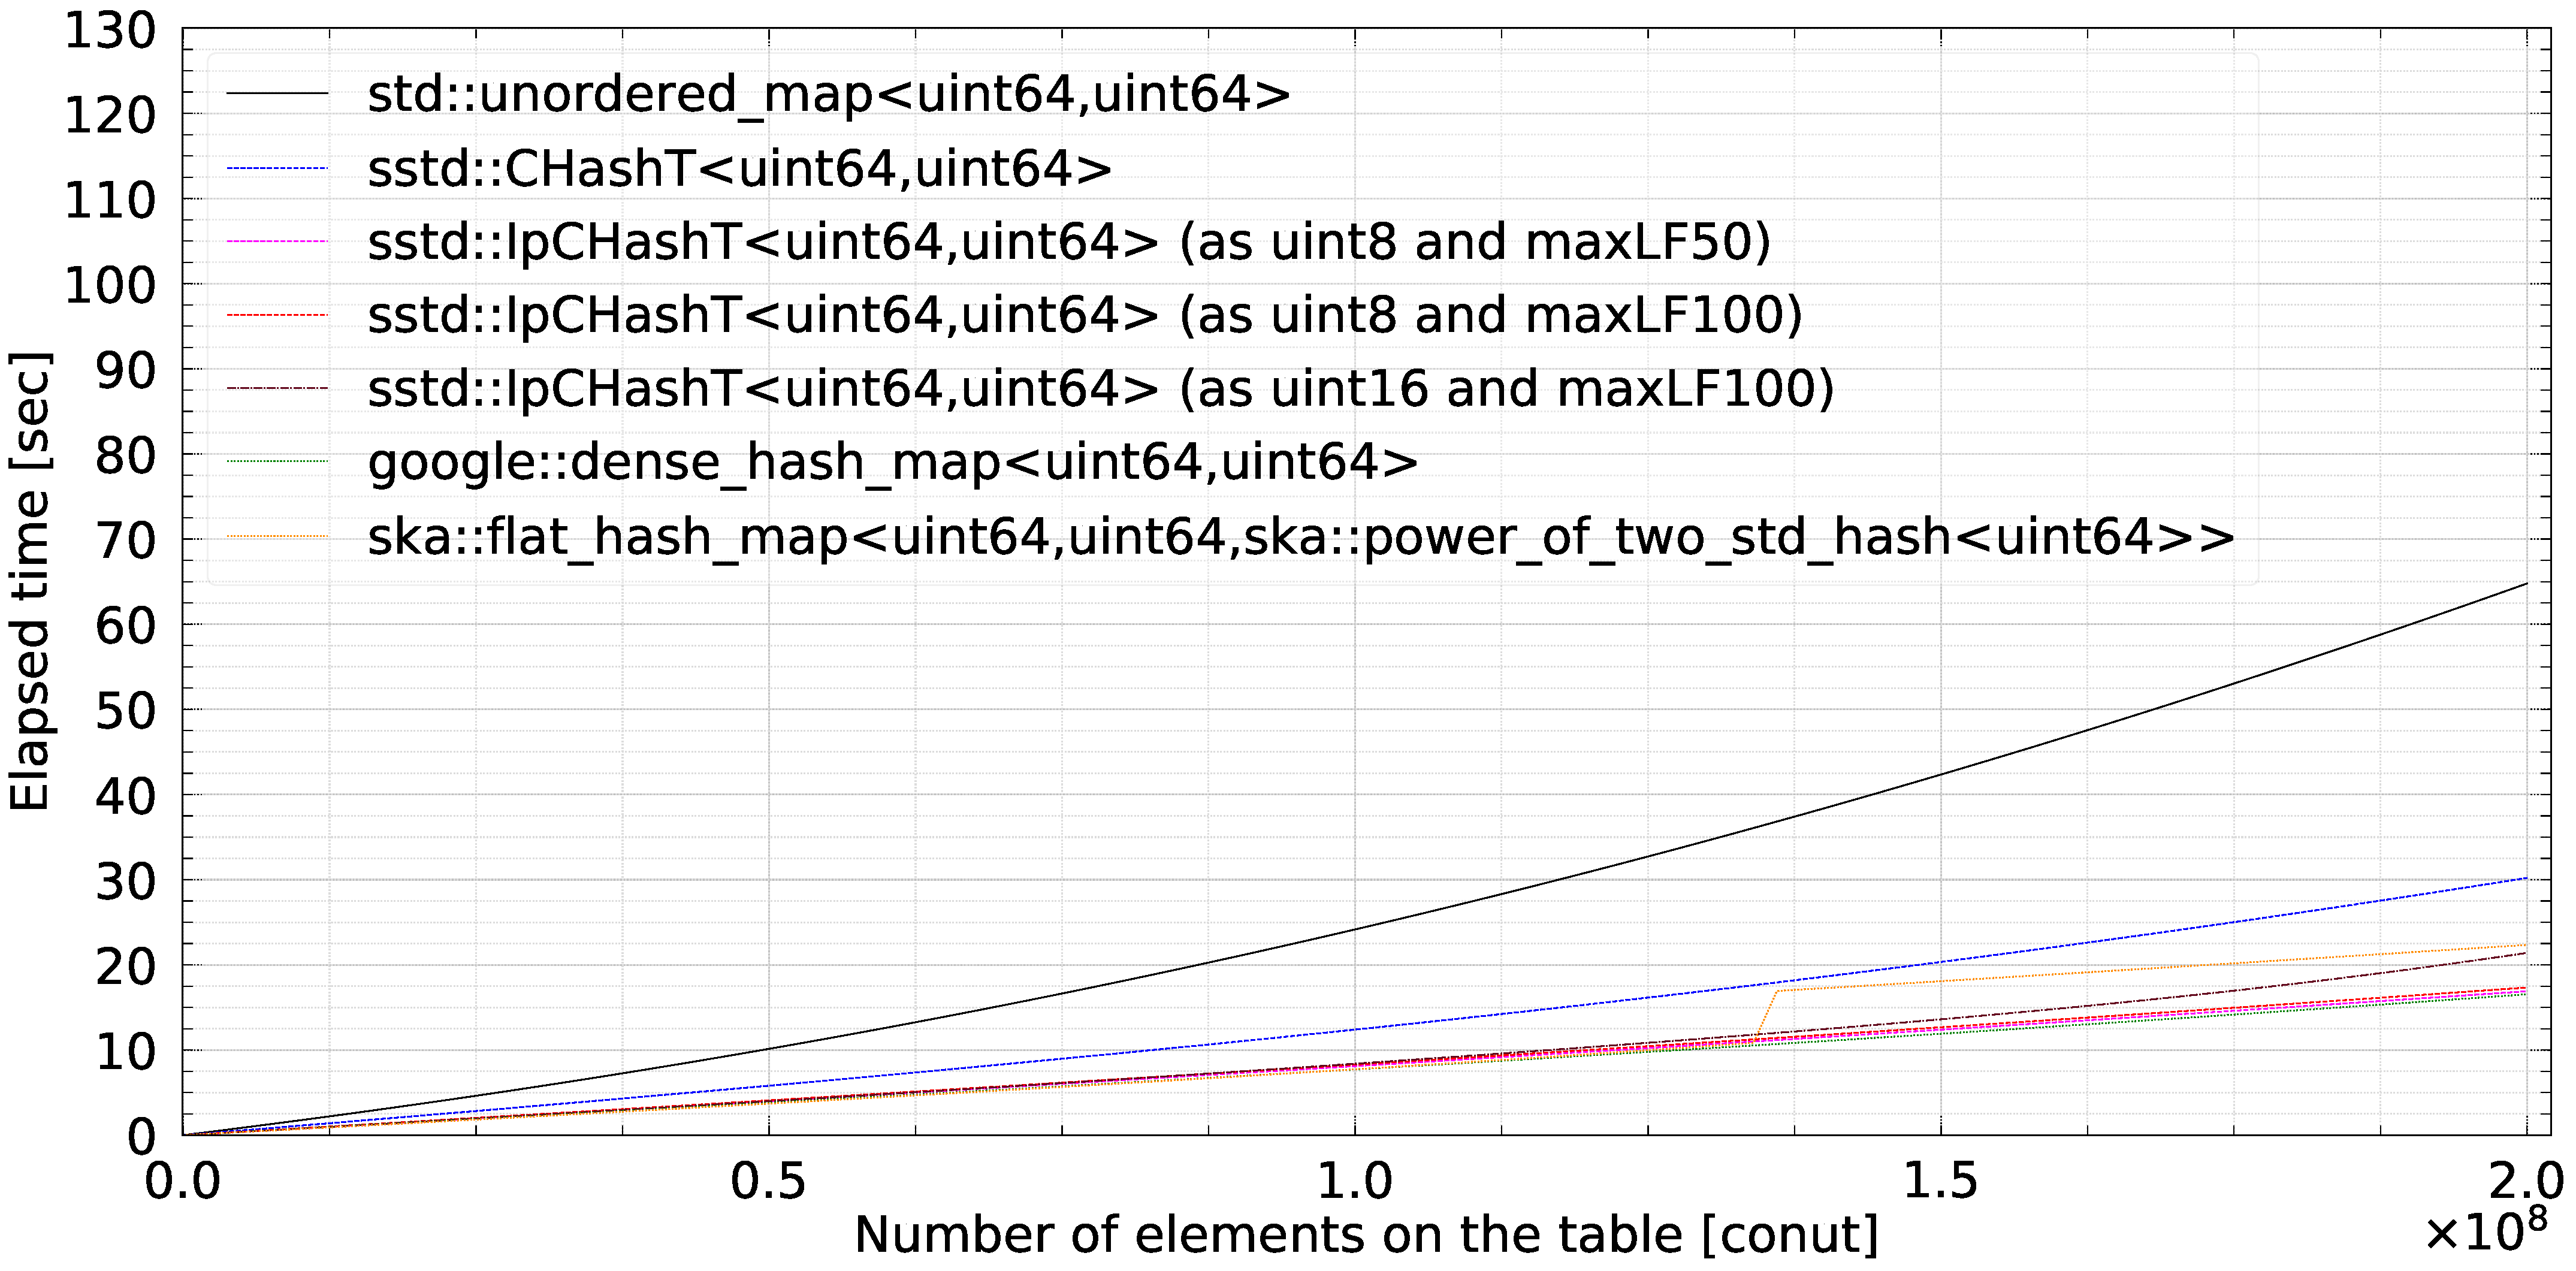
\includegraphics[scale=0.24]{./fig_bench/insert_et_preAlloc_med.pdf}
  \caption{ Total time of insertion using pre-allocated table. }
  \label{fig_bench_insert_preAlloc}
\end{figure}

\begin{figure}[h]
  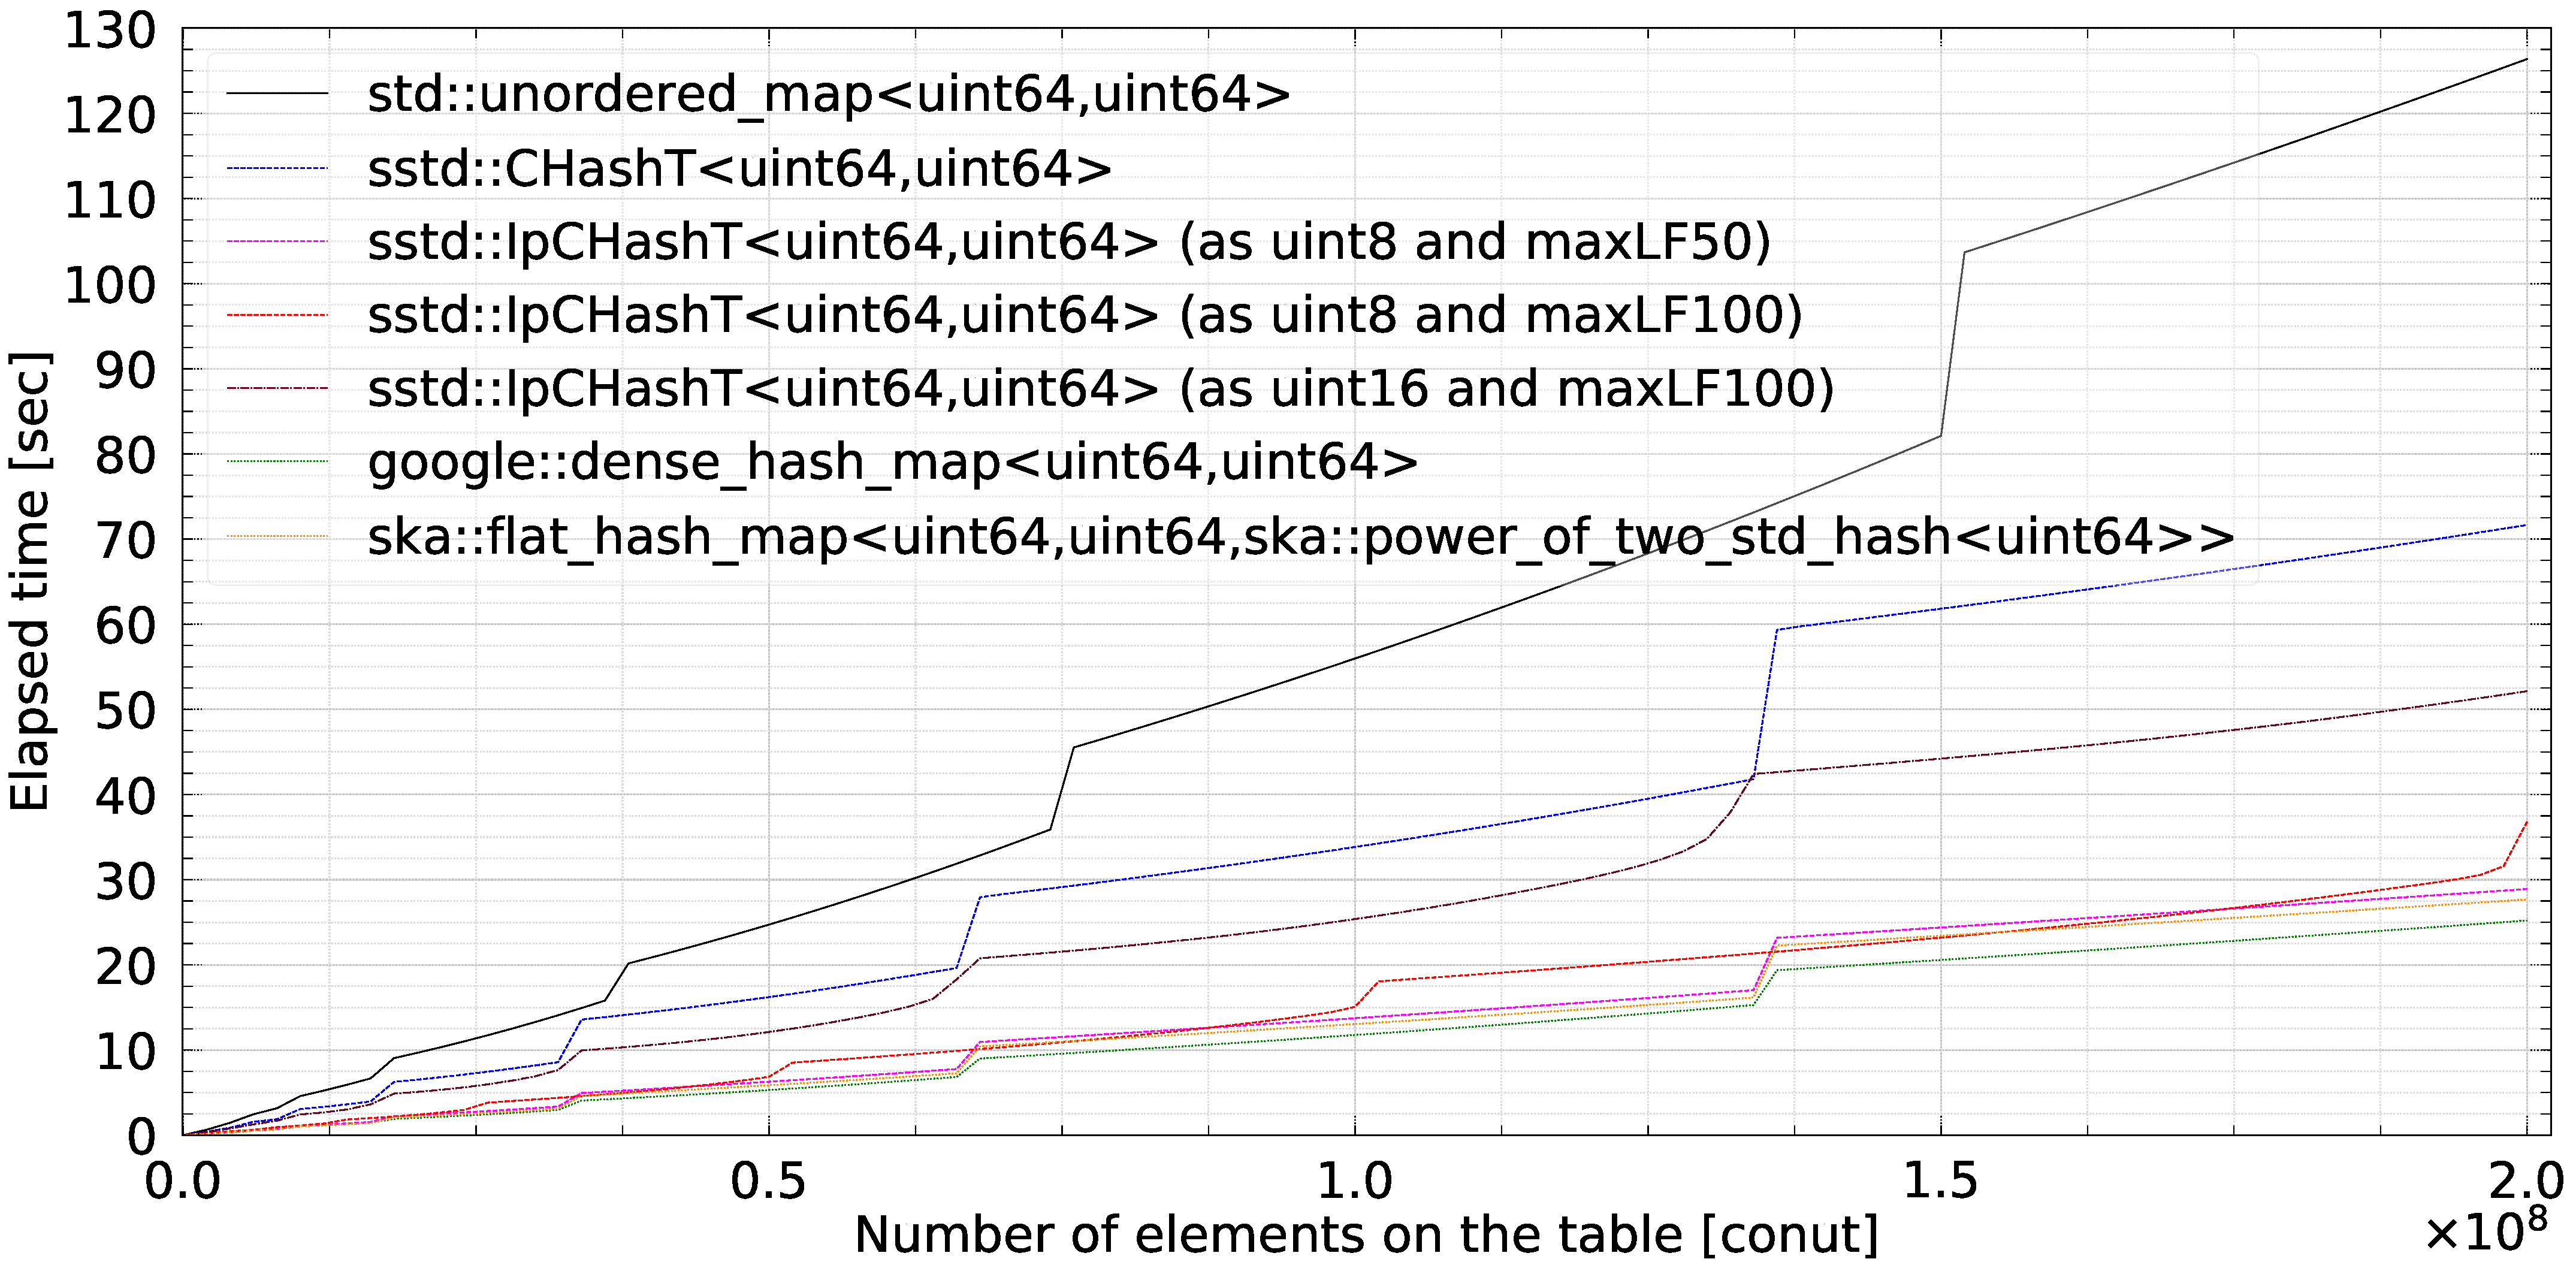
\includegraphics[scale=0.24]{./fig_bench/insert_et_med.pdf}
  \caption{ Total time of insertion with rehashing table. }
  \label{fig_bench_insert_wRehash}
\end{figure}

\begin{figure}[h]
  \hspace{-3mm}
  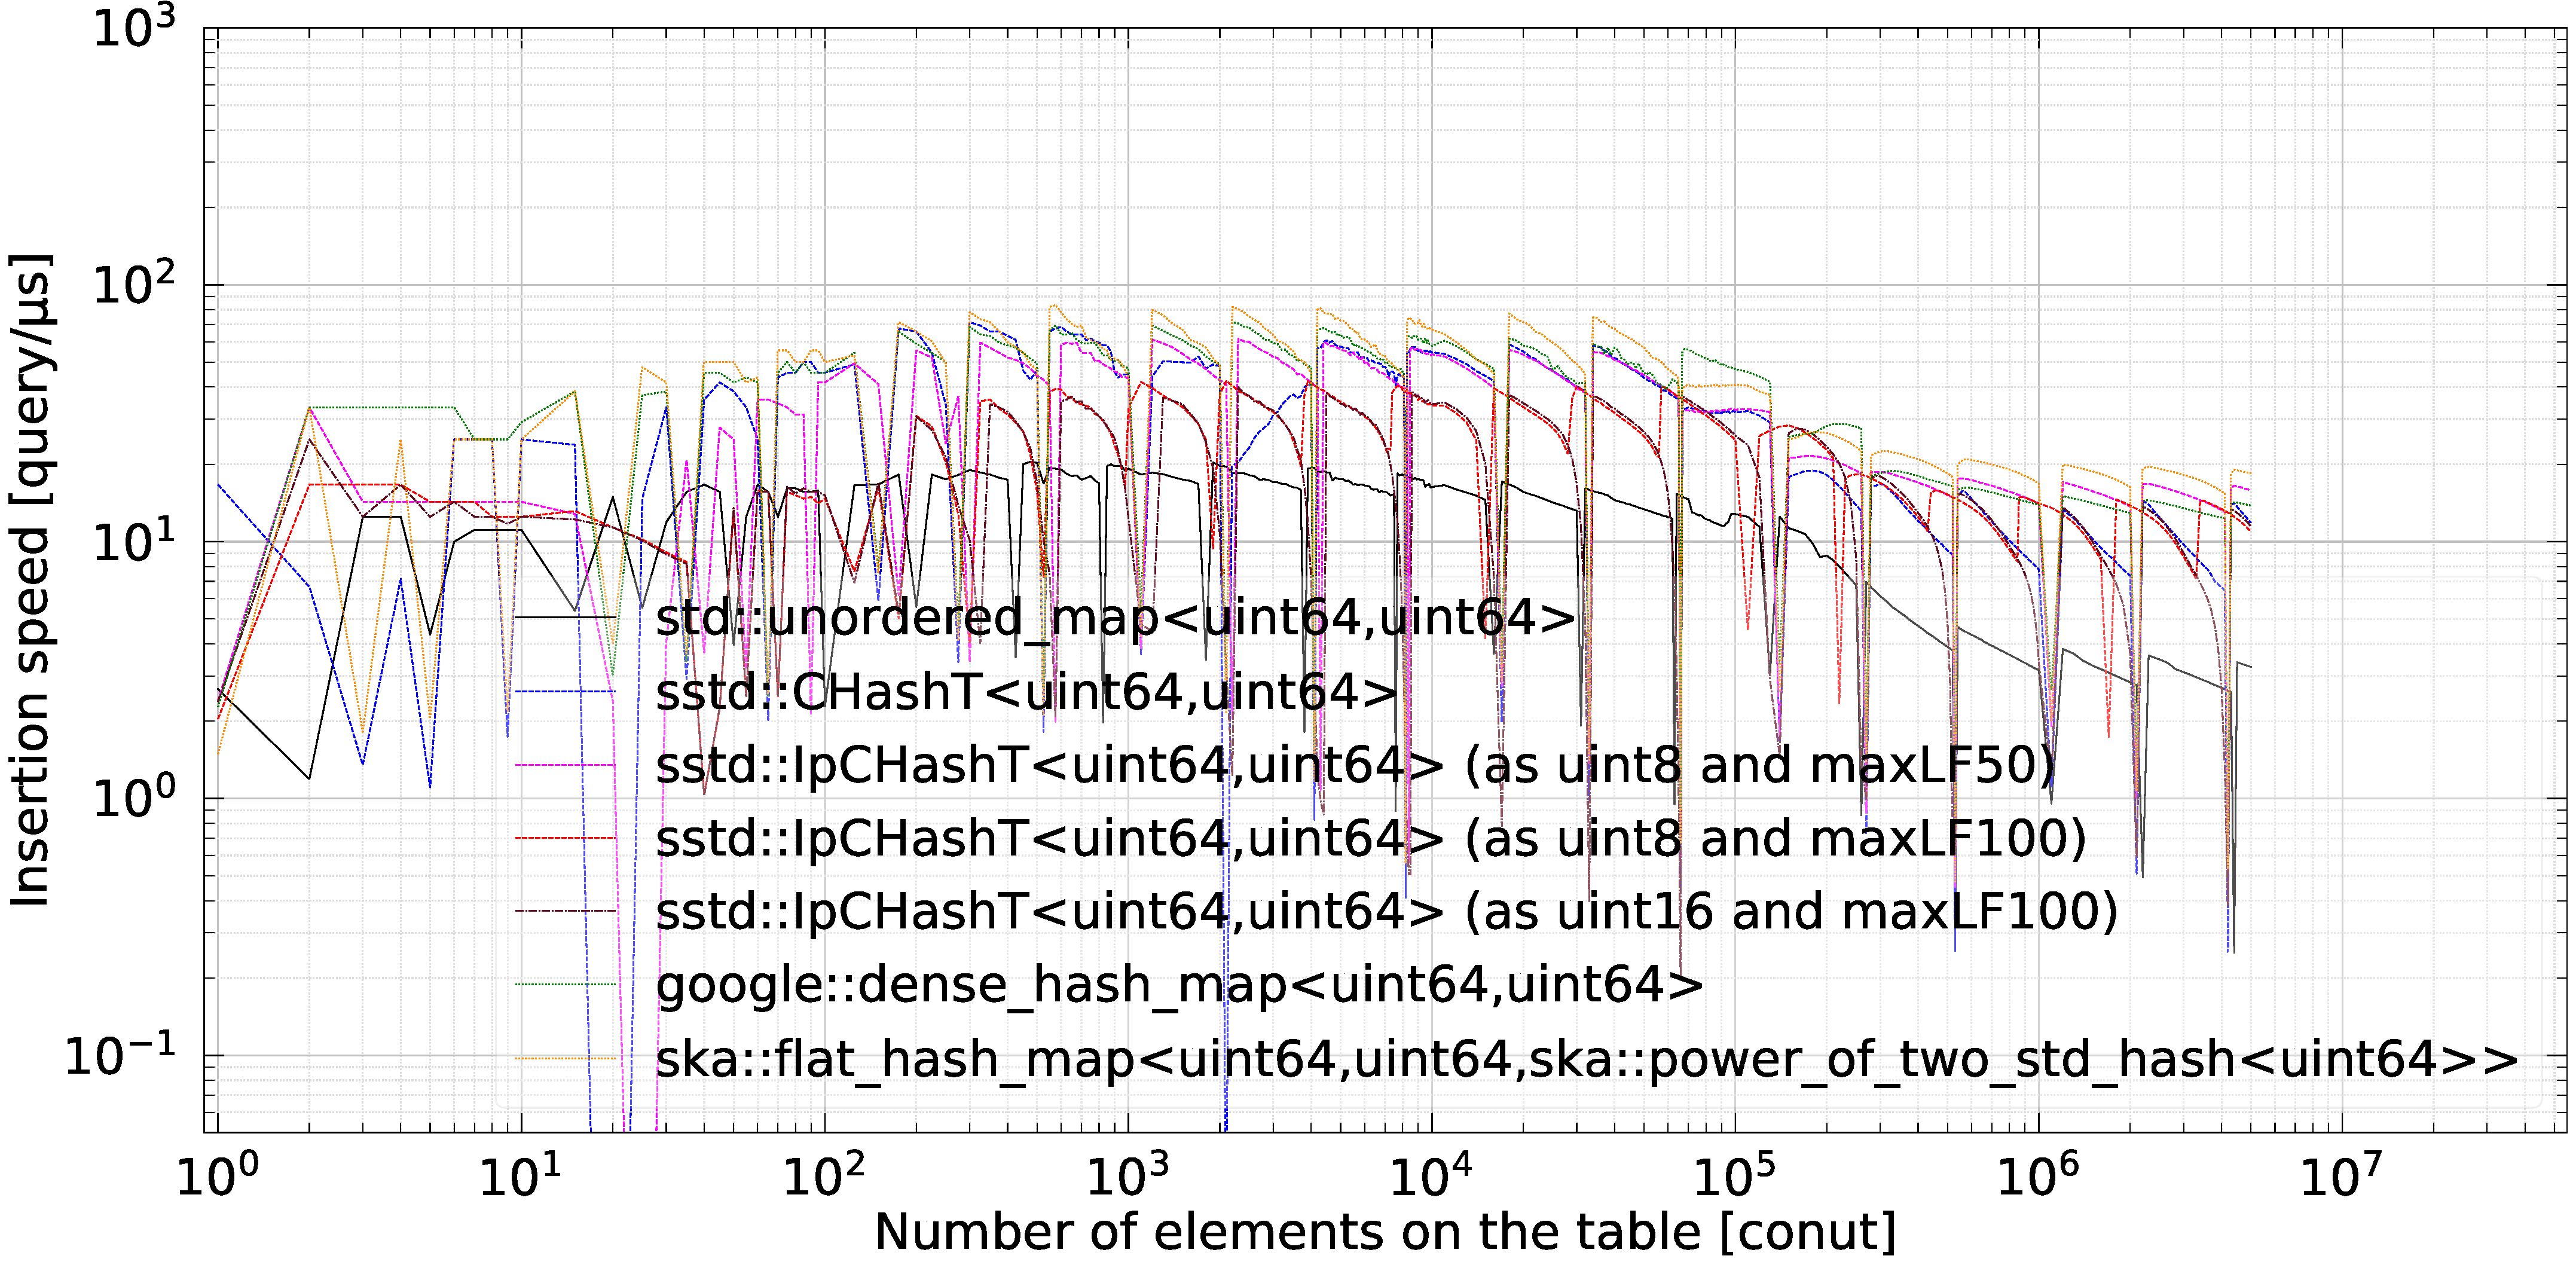
\includegraphics[scale=0.24]{./fig_bench/insert_med.pdf}
  \caption{ Insertion speed. }
  \label{fig_bench_insert}
\end{figure}

\begin{figure}[h]
  \hspace{-3mm}
  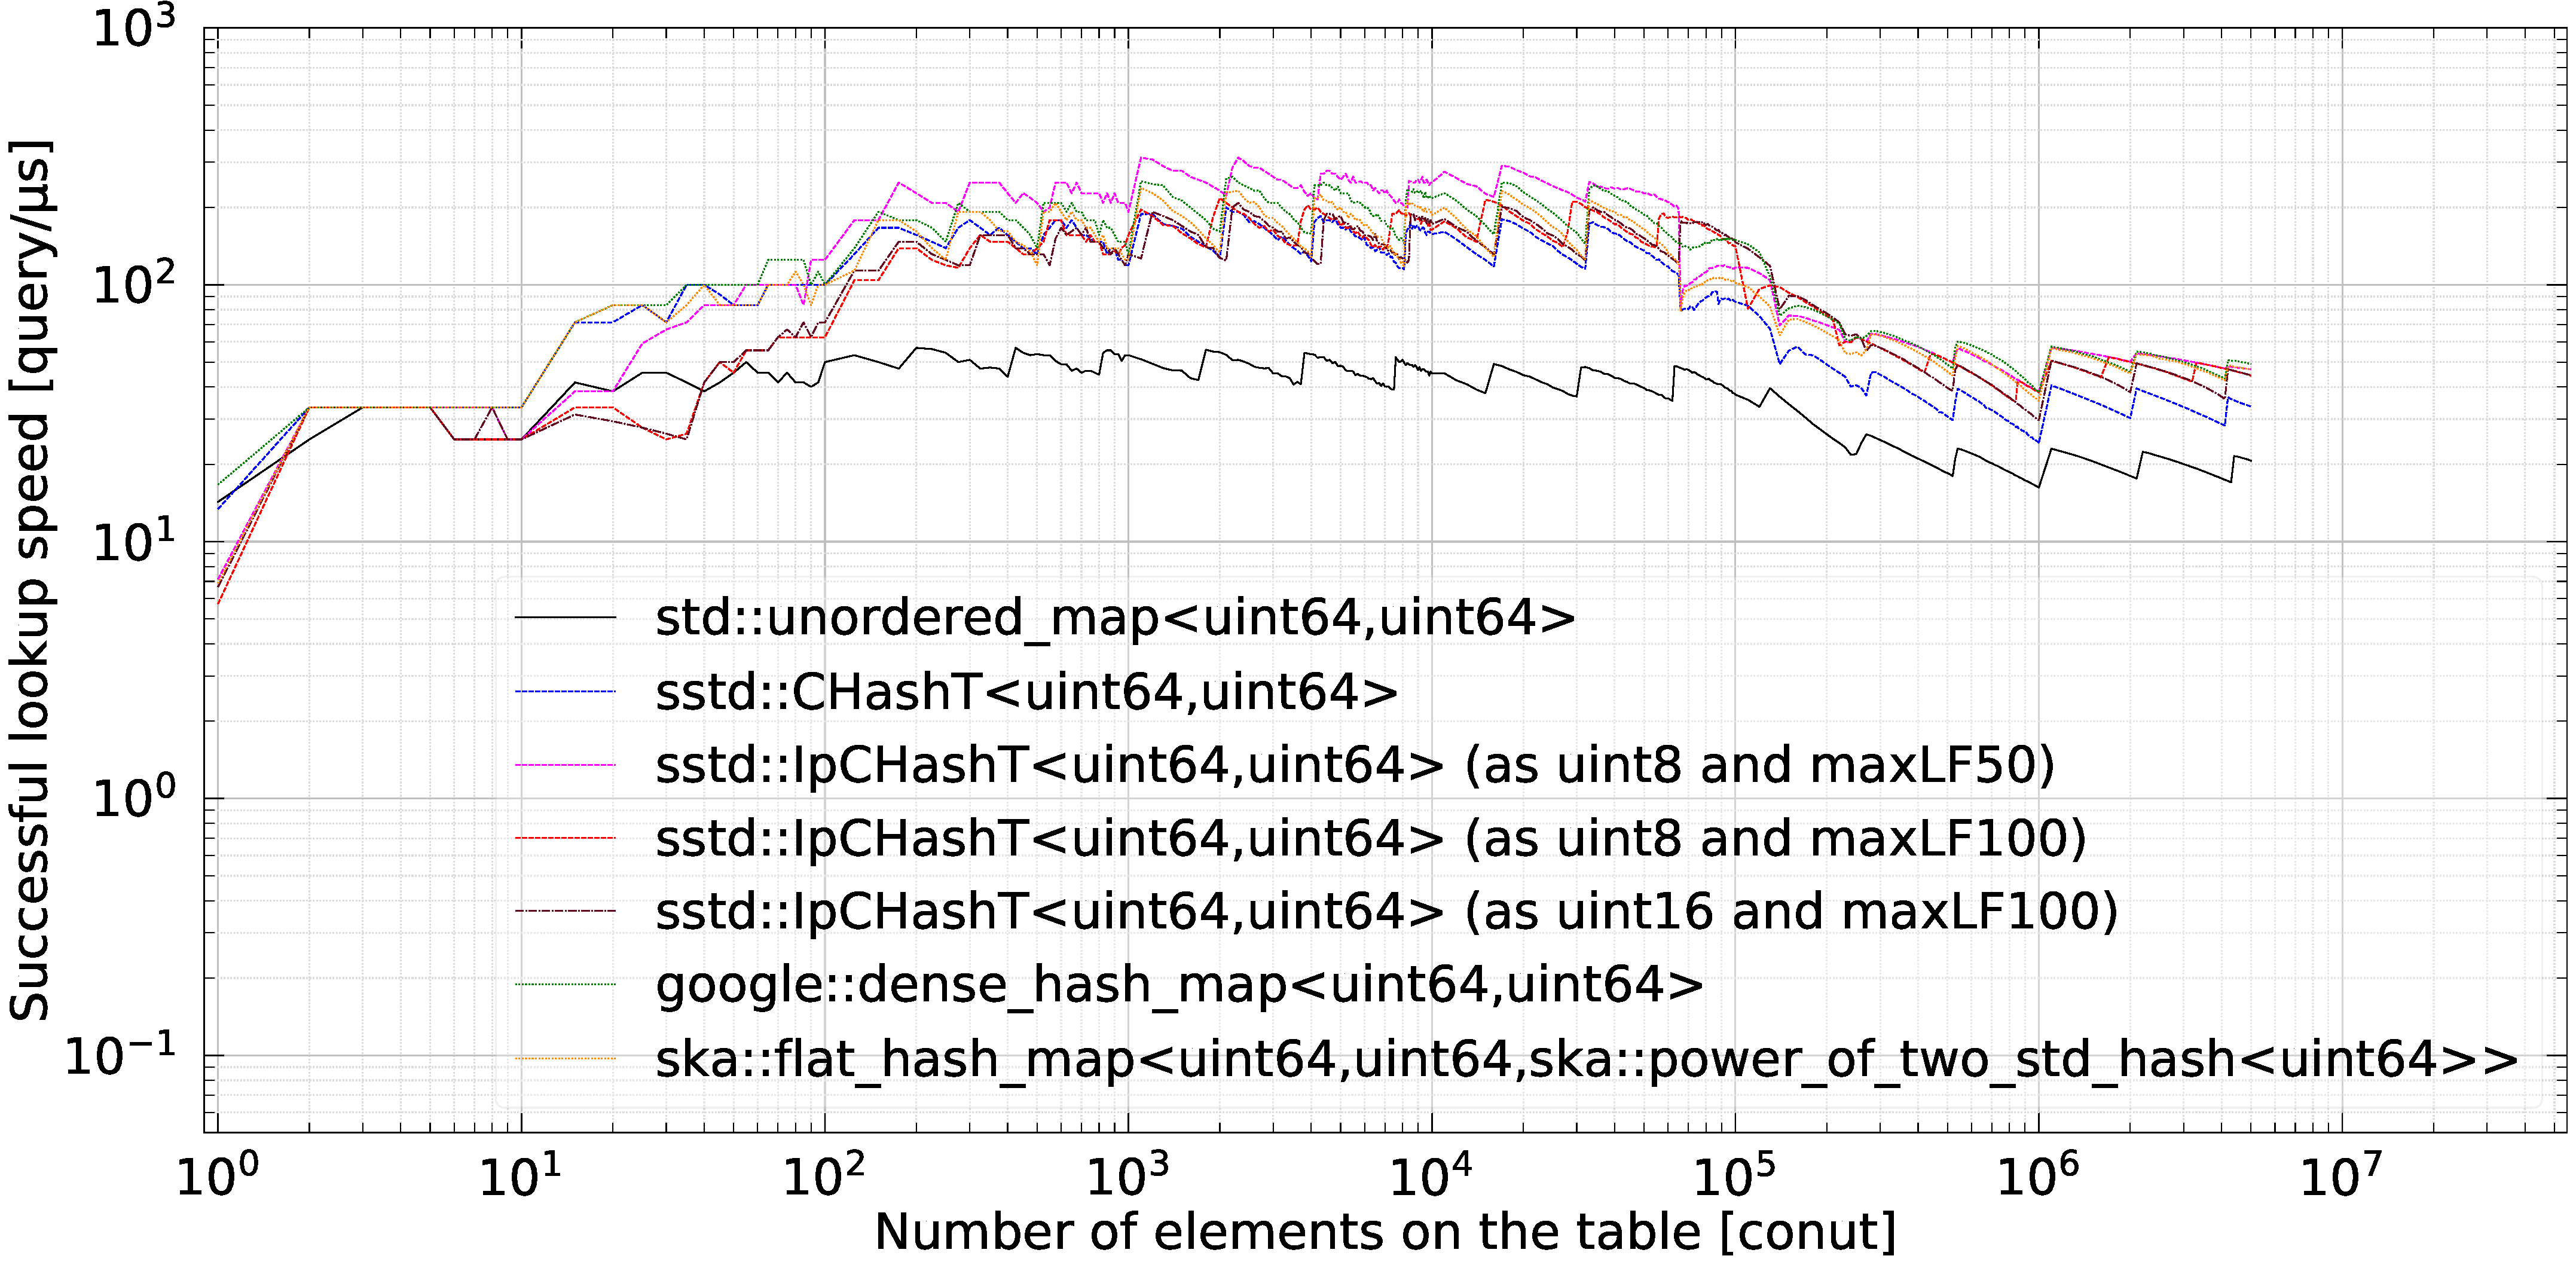
\includegraphics[scale=0.24]{./fig_bench/find_successful_lookup_med.pdf}
  \caption{ Successful lookup speed. }
  \label{fig_bench_insert}
\end{figure}

\begin{figure}[h]
  \hspace{-3mm}
  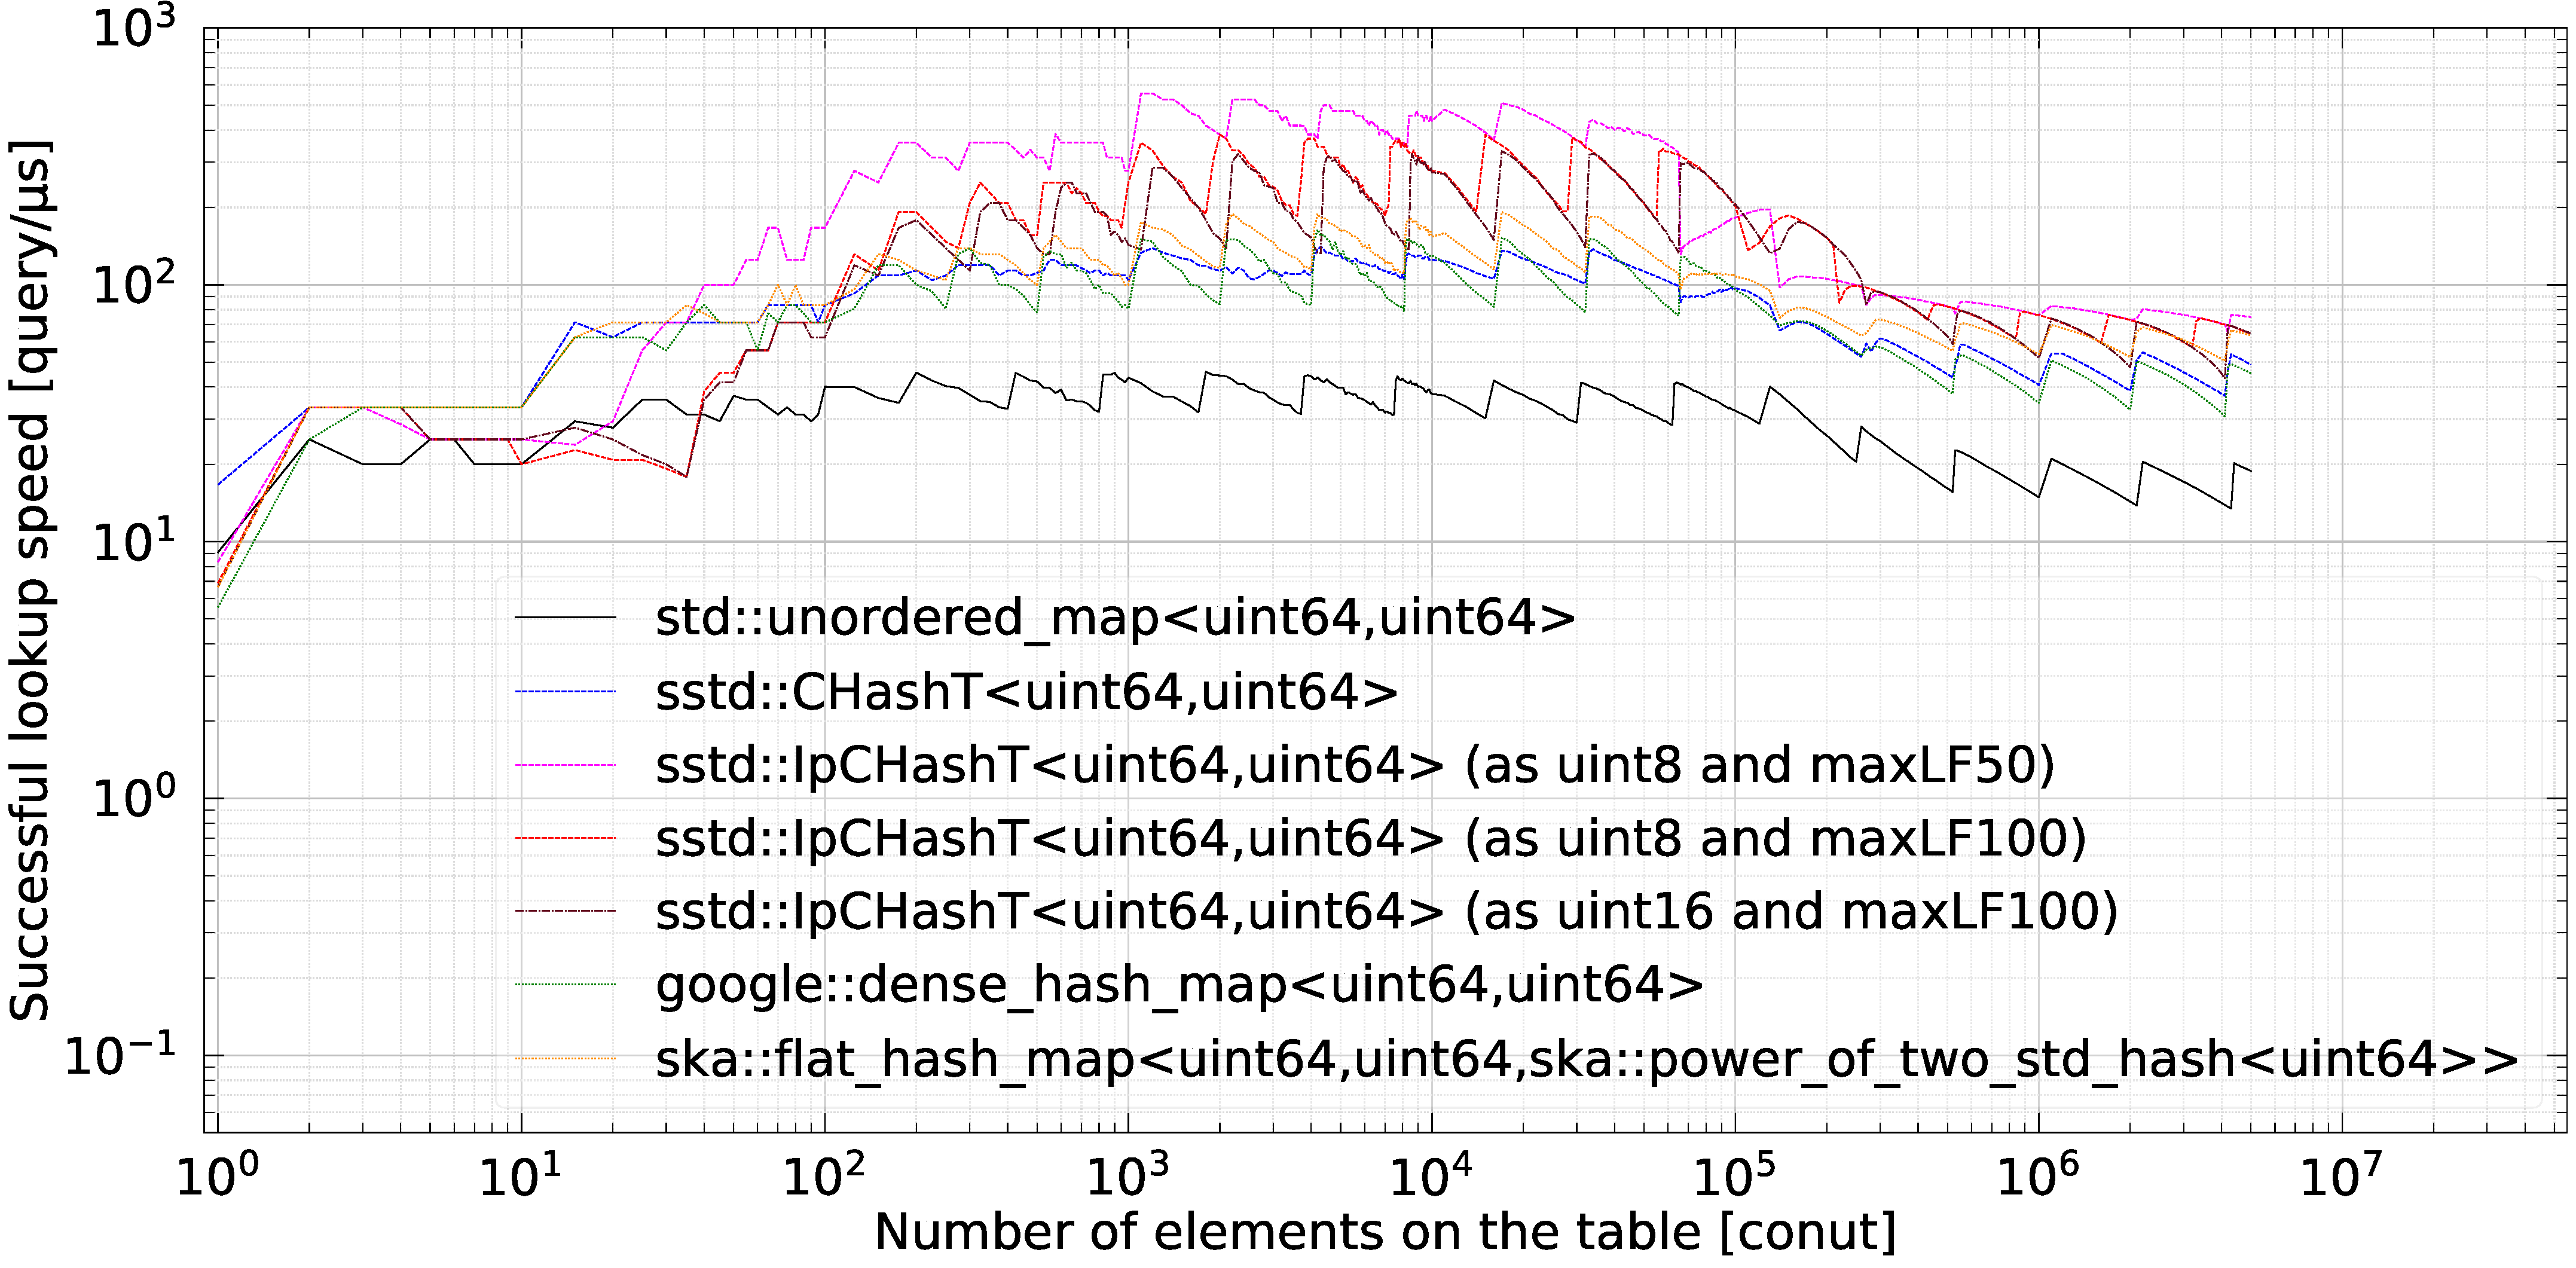
\includegraphics[scale=0.24]{./fig_bench/find_unsuccessful_lookup_med.pdf}
  \caption{ Unsuccessful lookup speed. }
  \label{fig_bench_insert}
\end{figure}

\begin{figure}[h]
  \hspace{-3mm}
  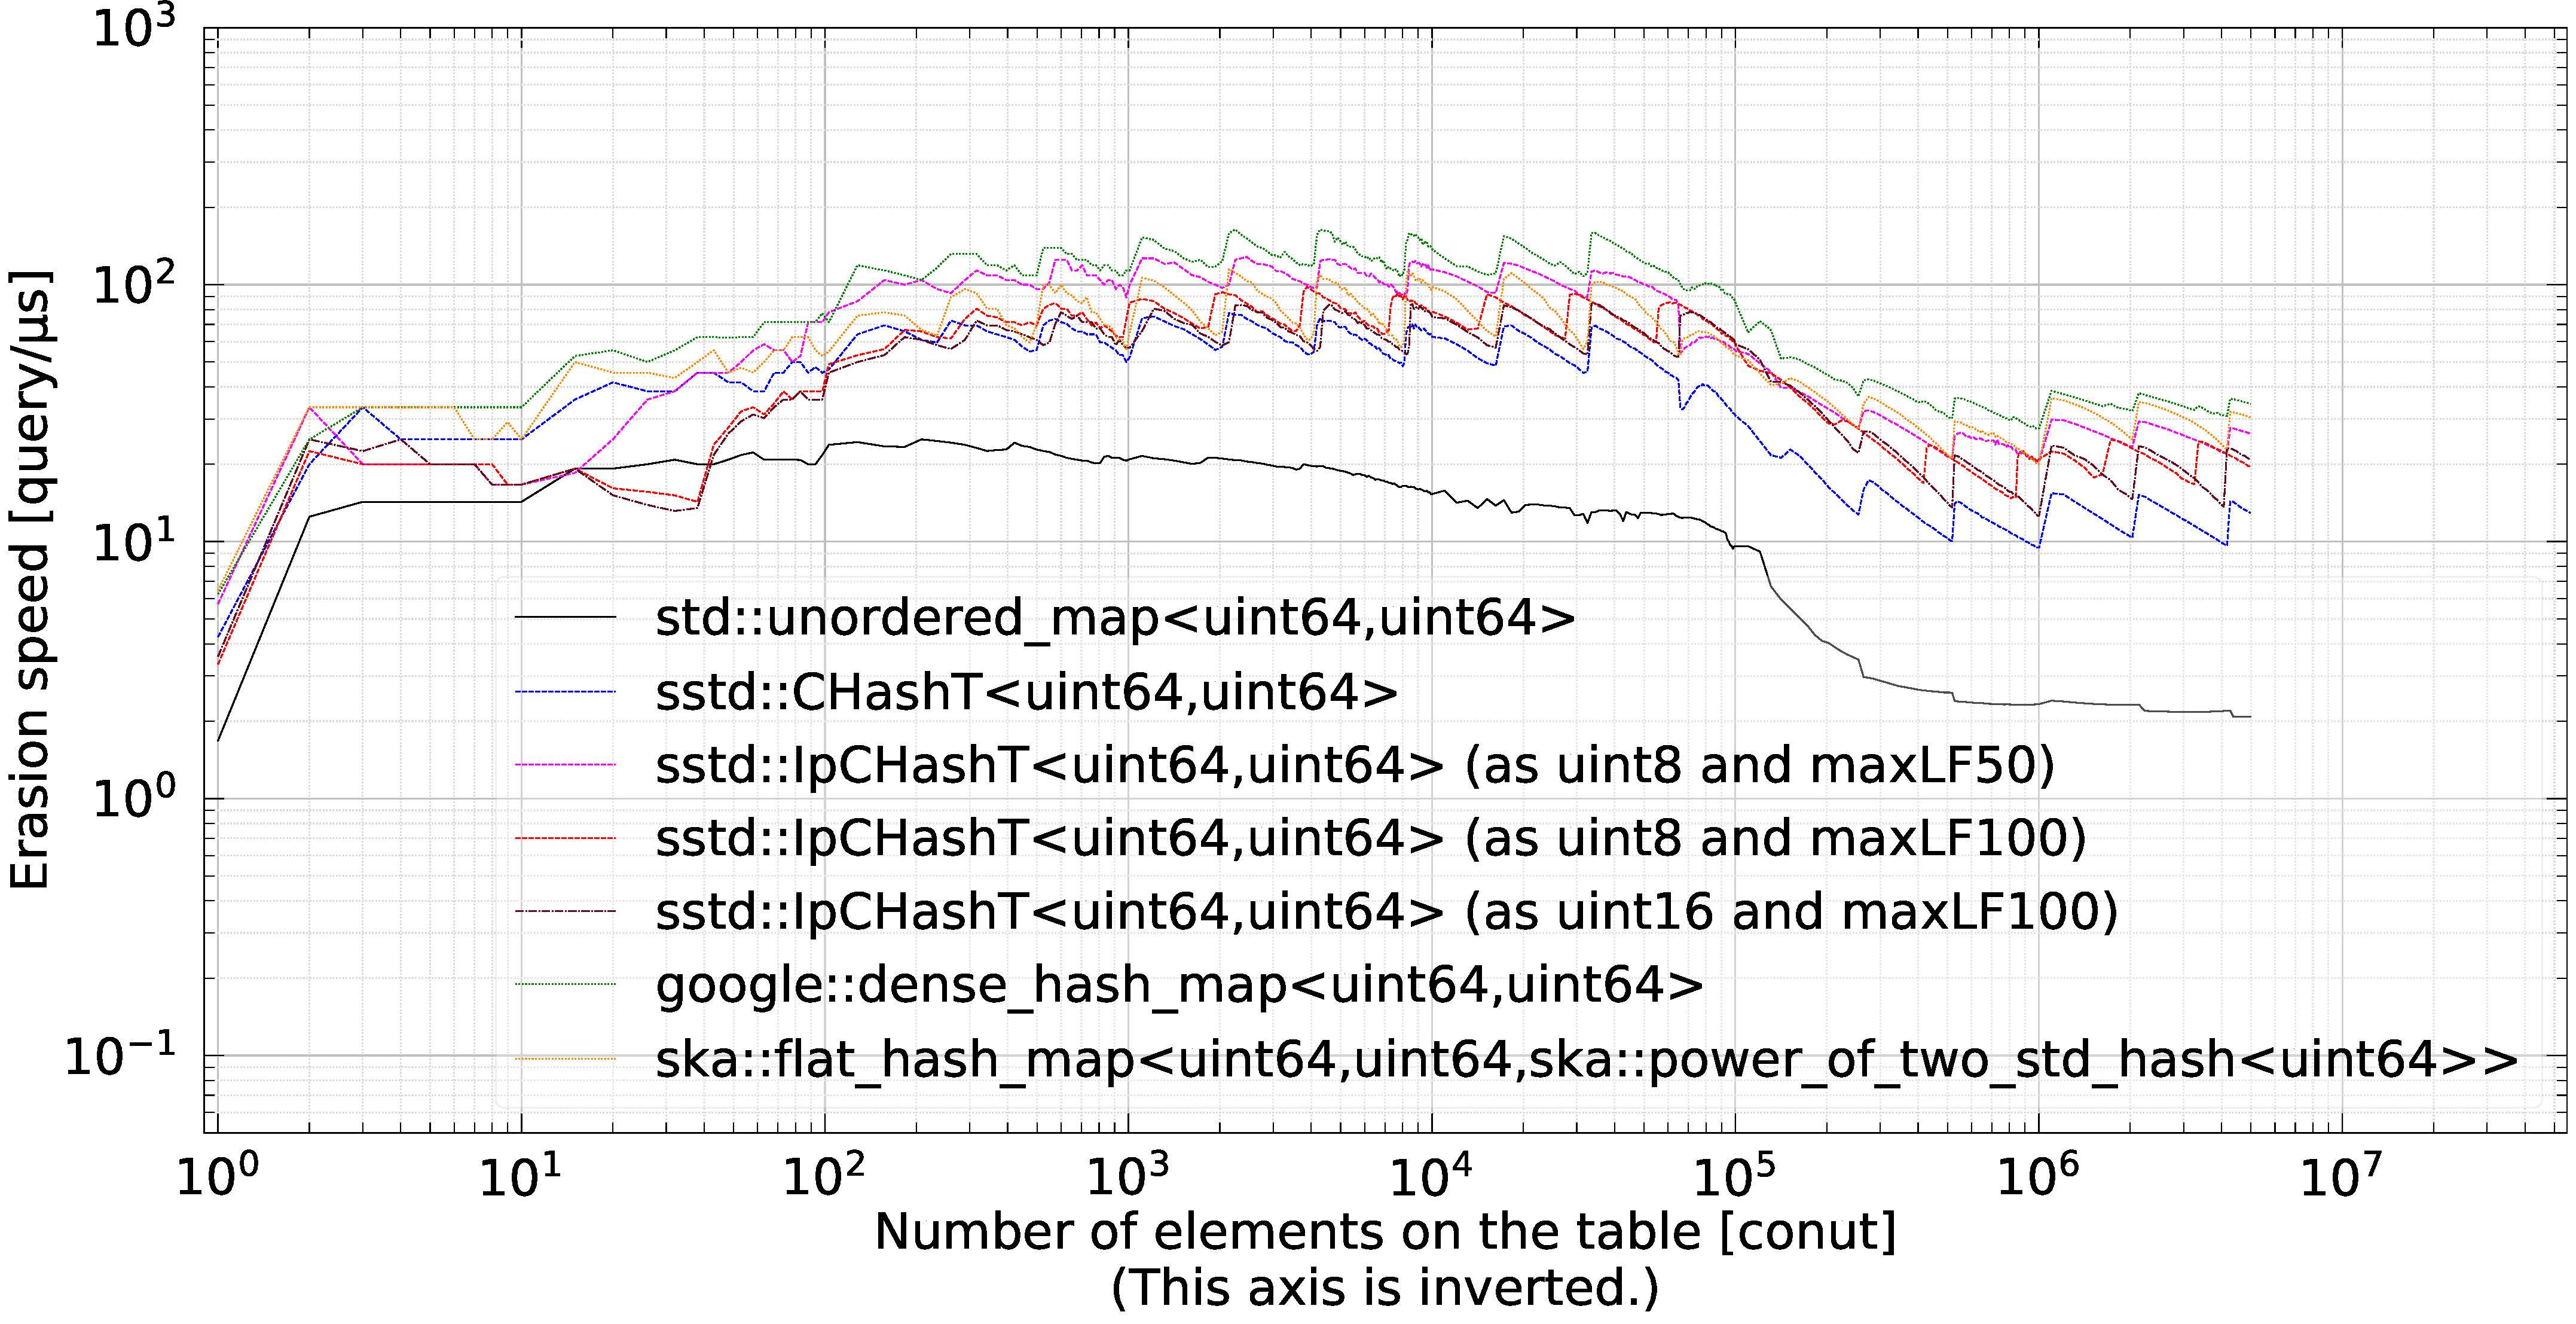
\includegraphics[scale=0.24]{./fig_bench/erase_med.pdf}
  \caption{ Erasion speed. }
  \label{fig_bench_insert}
\end{figure}
















